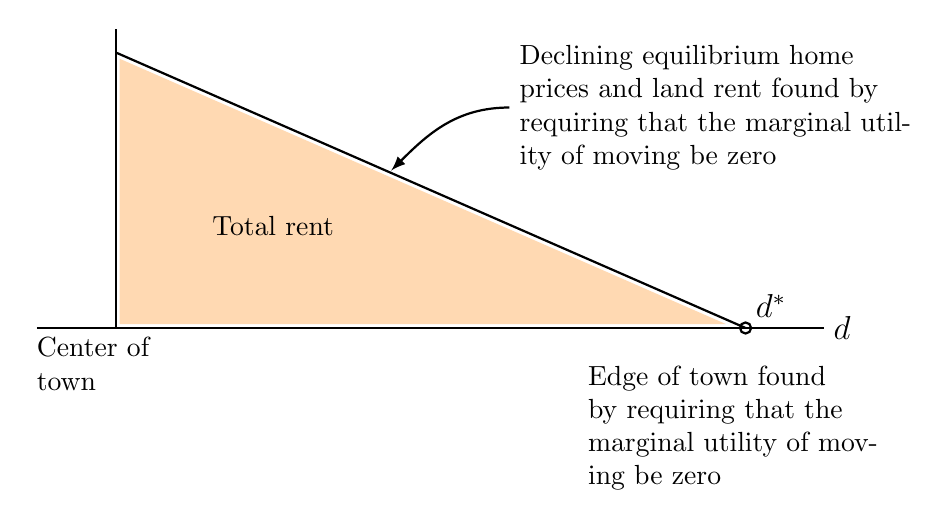
\begin{tikzpicture}[domain=0:2]
%\draw[thick,color=gray,step=.5cm, dashed] (-0.5,-.5) grid (3,3);
\draw[line width=.01] (0,0) -- (10,0) node[right] {\large $d$};
\node at (1,0) [below,text width=2cm] {Center of town};
%\draw[thick ] (0,3)node[above right] {merchant's price in town} -- (10,3) ;
\draw[thick ] (0,0)  -- (10,0); 
\draw[thick, -latex] (6,2.8)
node[right, text width=5cm]{Declining equilibrium  home prices and land rent found by requiring that the marginal utility of moving be zero} 
to [out=180, in=45](4.5,2); 

\fill[orange!30] (1.05,0.05)--(8.75,0.05)--(1.05,3.42)--cycle;

\draw[thick ] (1,0) -- (1,3.8);
\draw[thick ] (9,0)node [above right]{\large $d^*$}circle[radius=2pt] node[below=.35cm,text width=4cm] {Edge of town found by requiring that the marginal utility of moving be zero} -- (1,3.5) ;

\node at (3,1.3){Total rent};
\end{tikzpicture} 